\chapter{Technology Review}
About seven to ten pages.
\begin{itemize}
\item Describe each of the technologies you used at a conceptual level. Standards, Database Model (e.g. MongoDB, CouchDB), XMl, WSDL, JSON, JAXP.
\item Use references (IEEE format, e.g. [1]), Books, Papers, URLs (timestamp) – sources should be authoritative. 
\end{itemize}

%%%%%%%%%%%%%%%%%%%%%%%%%%%%%%%%%%%%%%%%%%%%%%%%%%
% Section - Docker
%%%%%%%%%%%%%%%%%%%%%%%%%%%%%%%%%%%%%%%%%%%%%%%%%%
\section{Docker}

\subsection{What is Docker?}
Docker is a platform that enables containerization of applications. Containerization provides standardized units for development, shipment and deployment. Container images are lightweight, isolated, executable packages of software that contain all the components to run the specified; the code, tools, dependencies, and settings. With availability on Linux and Windows based containers, both will run seamlessly regardless of the environment. Containers running in isolation means that regardless of how the environment or infrastructure which the container will run on, the application within the container will be unaffected by discrepancies across the environments, and other applications. Docker provides containers that run on a single machine share the operating system-kernel, resulting in rapid starting and less consumption of the central processing unit (CPU) and random access memory (RAM). Based on open standards, Docker containers can run on all major Linux distributions, Microsoft Windows, Apple MAC OS, and any infrastructure like: virtual machines, bare-metal, and via cloud services. 

\subsection{Docker Containers v Virtual Machines}
What are the benefits or differences of using Docker containers over Virtual Machines? 
While Docker containers and virtual machines have relatively similar resource isolation and allocation benefits, they function differently. Where a virtual machine will mimic the behavior of an operating system running on a physical computer, Docker containers visualizer just the operating system, rather than the operating system running on the hardware itself, resulting in higher efficiency and portability. Consider figure \ref{fig:containervsvm}

\begin{figure}
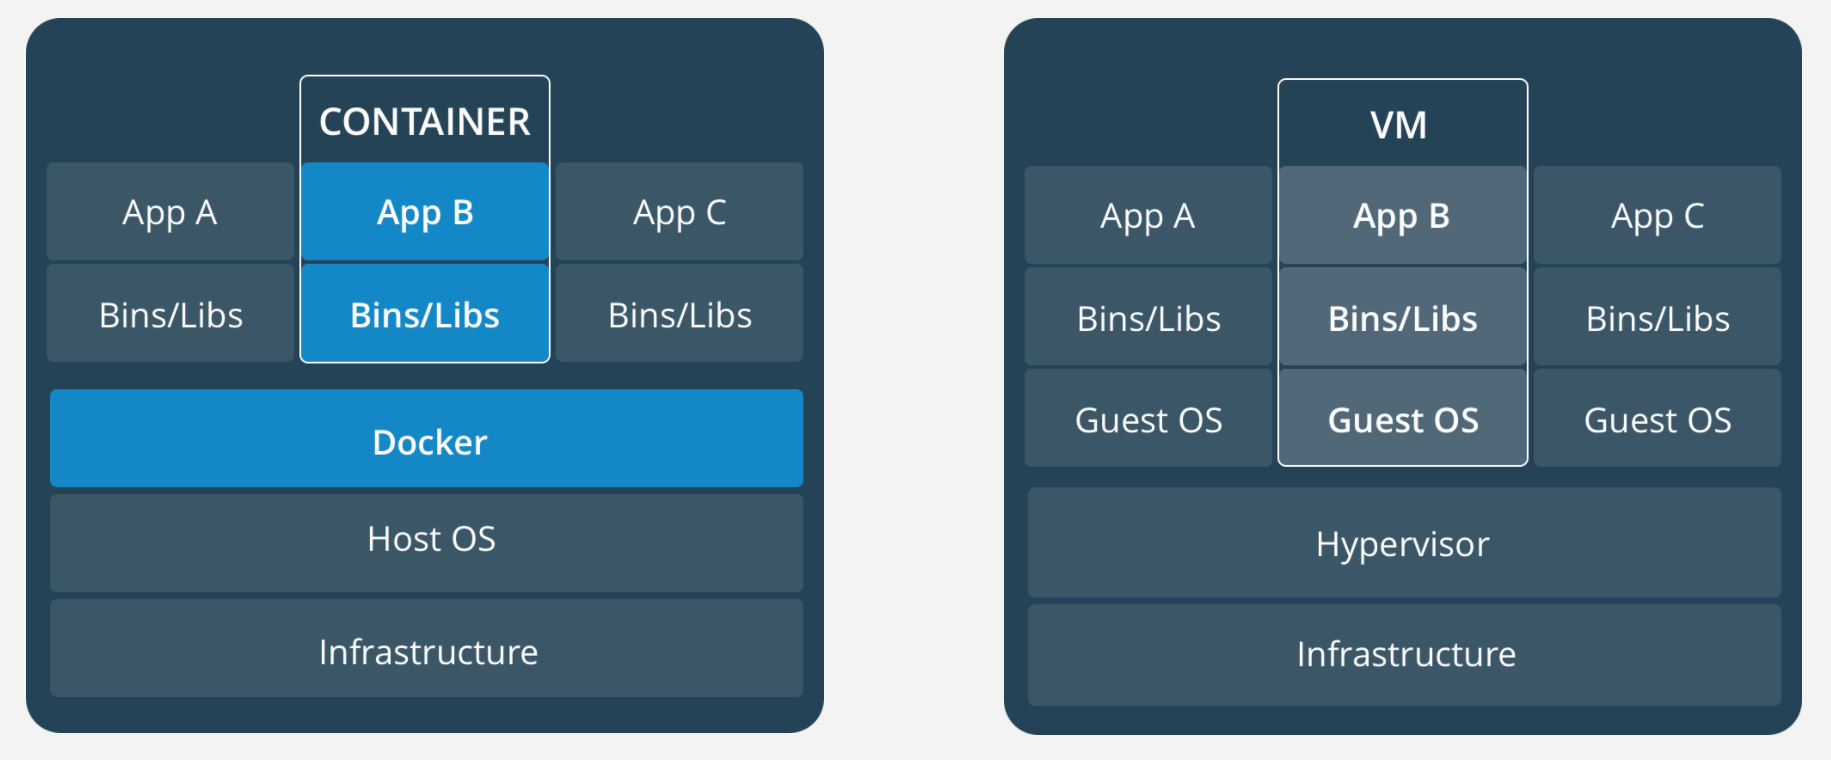
\includegraphics[width=\textwidth]{img/containervvm.PNG}
\caption{Docker Containers vs Virtual Machines}
\label{fig:containervsvm}
\end{figure}

Containers are an abstraction at the application layer which packages the code and dependencies  together. Numerous Docker containers can be running on the same machine and share resources such as the operating system kernel with other Docker containers running on the same machine, even though each of these Docker containers are running in isolation in the user space. Docker containers also require less space than virtual machines, with a container image typically using less than one hundred megabytes of storage space in size, alongside their near immediate start time.
On the other hand Virtual machines, are an abstraction of physical hardware allowing one server to appear or act as if it were many servers. The hyper-visor, also known as virtual machine monitor, produces any guest operating systems with a virtual operating platform and in turn manages the execution of all guest operating systems on the host machine. Each virtual machine will have a full copy of an operating system, one or many applications, any required dependencies, libraries and binaries, all of which would consume up to or more than one hundred gigabytes. Virtual machines can also be slow to launch. 

Docker is a container platform to construct, secure and administer a large array of applications from the early stages of development to deployment and production whether they are local or “in the cloud”. Docker Community Edition provides tools to build applications to developers for free, whereas Docker Enterprise Edition provides a Containers-as-a-Service platform for IT companies with multi-architecture operations at scale. 

\subsection{Dockerizing Existing Applications}
An application does not have to be built from the ground up with Docker, as existing applications  can be containerized. With potential of reducing cost, start up time, and provide a layer of security, Docker can aid in time and resource management when building new applications or even modernizing legacy applications. Using the Modernize Traditional Applications [MTA] kit via Docker Enterprise Edition, developers can package existing applications into containers, which will enable the application to be portable. This alteration implements modern properties to legacy applications, without the need to change any of the source code. It will also reduce the overhead required to run the legacy application, increase operational efficiency, and consolidate infrastructure.

Because Docker packages applications and their dependencies together into an isolated container, this makes them portable to any infrastructure, making them suitable for Cloud migration, multi-cloud or hybrid cloud infrastructures. Thus eliminating the age-old “works on my machine” problem. The Docker Certified Infrastructure guarantees that the containerized applications work consistently. It provides an integrated environment for multiple distributions of enterprise Linux, as well as on Cloud providers such as Amazon Web Services, Azure and IBM. Docker Certified containers provide trusted independent software vendor products packaged and distributed via Docker containers. Docker Certified plug ins provide easy to download and install containers for an environment, as well as networking and volume plug ins.

\subsection{Continuous Integration and Services}
Docker also provides tools and strategies to Developer Operations (Dev Ops) teams. John Willis’ White paper on “Docker and the Three Ways of DevOps“, outline three principles known as “The Three Ways of DevOps”, and describes the purpose of these principles, how to apply these principles using Docker within organizations, and the results and benefits from doing so. 

\textbf{\emph{“The First Way: System Thinking”}}

This is referred to as the pipeline; the flow and direction from left to right, outlining the importance of understanding the system as a complete value stream. Managing this concept is often referred to as bottleneck reduction or global optimization, or “Lead Time” in the Lean project management methodology\cite{willis}. This is the equivalent of the time taken to get from rough diagrams to the delivery of a product to paying consumers, or in simpler terms, the time from starting a project, and the project becoming a product of value\cite{willis}.  To ensure System Thinking is effective, Dev Ops teams need to able to apply the following:

\begin{itemize}
\item Escalate “velocity” by hastening each process component within the pipeline.
\item Diminish “variation” by removing wasteful or time intensive sub processes within the pipeline.
\item Ascension of processes by isolating functionality, therefore improving visualization and understanding of the overall flow.
\end{itemize}

Docker can aid the above in the following ways:
\begin{itemize}
\item \textbf{Velocity:}
	\begin{itemize}
	\item In regards to \emph{Development flow}, developers using Docker can create Docker environments locally on their machine to develop and test containerized applications. In contrast, the alternative of using virtual instances running as numerous hosts could consume a lot of time during start up time and convergence, depending on the overall complexity\cite{willis}. To summarize, Docker delivers less context switching time for testing and retesting, resulting in significantly higher velocity.
    \item In regards to \emph{Integration flow}, Docker can simplify continuous integration with use of Dockerized build slaves.  A continuous integration system can be designed in such a way that it would allow multiple virtual instances to run in isolation, each as individual hosts. Environments can run Docker hosts within a Docker host, termed “Docker-in-Docker” for build environments. This provides elegant isolation of the build and breaks down the environments for the services in test, meaning that the original instances are never debased due to the embedded host having the ability to be recreated for each slave instance\cite{willis}. 
    \item Finally with regards to \emph{Deployment flow}, to achieve higher velocity in  Continuous Delivery of software, there are numerous approaches that may be hit by using Docker. One challenge of production deployments is ensuring the seamless and quick changeover time from version to version. "A Blue Green deploy is a technique where one node of a cluster is updated at a time (i.e., the green node) while the other nodes are still untouched (the blue nodes)."\cite{willis} This approach requires a continuous process where each node is updated and tested, one at a time. The fundamental outcomes  of this are:
	\begin{enumerate}
		\item The time required to update all nodes needs to be fast.
    	\item If a cluster requires roll back, this must also be done fast.  
	\end{enumerate}
    To summarize, Docker containers execute the roll back and roll forward processes more efficiently, and also are a lot cleaner due to container isolation during changeover.
	\end{itemize}
\item \textbf{Variation:}
	A fundamental pro of using Docker images throughout the software delivery pipeline is that the environment and application can both be packaged within the container image. With Docker, a developer can package the actual environment (e.g OS, dependencies, other requirements) within the same image. This convergence reduces the possible variation at all stages of the delivery pipeline; i.e. development, integration, and  deployment\cite{willis}. If a developer were to test a collection of Docker images as a service on any machine, the services in question can be the exact same during integration testing and right up to deployment. "A Dockerized pipeline approach delivers converged artifacts as binaries and therefore are immutable starting from the commit"\cite{willis}.
\item \textbf{Visualization}
	Containerized Microservices is a model which has been generating a buzz within the software development world lately. In an architecture of micro services, “services” are defined as bounded context. When these services are connected as Docker containers and used within the delivery pipeline, they become visible without delay on a domain. Services become more visible in the pipeline when bounded by their business context and then isolated as Docker containers. With more visibility an organization can isolate, and determine control rapidly; thus reducing overall Mean time to repair\cite{willis}.
    "The “First Way”” and Docker can provide global optimization around software Velocity, Variation and Visualization. Dockerizing the development pipeline, organizations can reduce the cost and risk of software delivery while increasing the rate of change."\cite{willis} 
\end{itemize}

\textbf{\emph{"The Second Way: Amplify Feedback Loops"}}

"The "Second Way" is defined as amplifying and shortening feedback loops such that connections can be made fast and continuously."\cite{willis} also known as the right to left flow.

\begin{itemize}
\item \textbf{Velocity}
	In the second way velocity means the same as Velocity from the first way. The flow in this case may not always be going in the same direction. Defect cause interruptions in the flow and changeover time. Dev Ops need to manage, feedback, changeover speed, the adaptiveness of the system in relation to defect detection, and reimplementation. Dockers streamlining of packaging allows organizations to utilize shorter changeover times because of defects, making it easier to halt processes if any defects are indeed identified.\cite{willis}
    \item \textbf{Visualization}
    An advantage of the immutable delivery process is most artifacts are conveyed throughout the pipeline as binaries\cite{willis}. This means that service delivery teams are able to generate meta-data from the source that is maintained, enabling visualization at any stage within the pipeline. With that meta-data the time required to resolve defects is reduced, therefore the overall Lead Time of the service being delivered is also reduced. 
\end{itemize}

\textbf{\emph{"The Third Way: Continuous Learning"}}

"In this “Third Way”, the symbol of a complete loop is used because it ties the first two ways together through a rigorous implementation of a learning process."\cite{willis} The word Kaizen is often seen as an approach of continuous improvement within an organization. This approach being fulfilled through a culture of continuous experimentation and learning in all parts of the organization\cite{willis}. The speed to market is essential in the deliverance of software and services. It is also the speed at which reaction, and reproduction to customers validation of the delivered service. The major principles of the Dev Ops mindset all point to outcomes like rapid innovation, increased quality and a feedback loop of continuous learning. "The Docker platform uniquely allows organizations to apply tools into their application environment to accelerate the rate of change, reduce friction and improve efficiencies."\cite{willis}.

\subsection{Conclusion}
	To summarize, Docker as a development tool is relatively easy to pick up and implement, due to the fact that it is well supported and documented by its community. However, it comes with a steep learning curve as you traverse deeper into its more advanced features and functionality. The isolated environments that Docker containers provide, enables work across different machines regardless of the underlying infrastructure, which in the case of this project, provided an easy work flow during cross examination, merging, and service integration. Going forward Docker will continue to make this project more and more versatile, secure, quick, and easy to maintain because of the Docker ethos. Long after the project has been deployed and it is in use by the product owner, integration engineers and developer operations teams should find processes like: onboarding new services, or analyzing and repairing problematic services easy to identify, then address, seamlessly and fast. Finally with the exponential growth in adoption rate of Docker over the last couple of years, virtual machines may very well be a thing of the past in years to come.

%%%%%%%%%%%%%%%%%%%%%%%%%%%%%%%%%%%%%%%%%%%%%%%%%%
% Section - Node.js
%%%%%%%%%%%%%%%%%%%%%%%%%%%%%%%%%%%%%%%%%%%%%%%%%%
\section{Node.js}
\subsection{About Node.js}
	Node.js or more commonly referred to as Node is designed as an asynchronous event driven JavaScript runtime for scalable network applications built off Google Chrome V8 Engine. Google Chrome V8 Engine will translate the JavaScript, which Node Application Programming Interface's are written in, into machine readable code. Node provides the ability to handle many connections concurrently using callbacks, but if there is no work pending, it will sleep\cite{node}. This is in opposition to the current common concurrency model that employs operating system threads, as thread-based networking can be relatively difficult to use and inefficient. Node users need not worry of processes dead-locking, since no locks exist. I/O processes never block, because very few functions in Node directly perform I/O, as a result of this scalable systems are feasible to build using Node. Node presents an event loop as a runtime construct rather than as a library. Node will enter this event loop after execution of an input script, and exit the event loop once all callbacks have been performed\cite{node}.
    
\subsection{JavaScript to Machine Code via the Google Chrome V8 Engine}
	\subsubsection{Overview}
    	The V8 Engine is an open source high-performance JavaScript engine from Google, written in C++ that is used in Google Chrome, Node, and more. The V8 Engine can be embedded into any C++ application or run standalone\cite{googleV8}. \emph{"V8 implements ECMAScript as specified in ECMA-262, 5th edition, and runs on Windows (XP or newer), Mac OS X (10.5 or newer), and Linux systems that use IA-32, x64, or ARM processors."}\cite{googleV8} 
	\subsubsection{Technical details}
    The V8 Engine is capable of compiling and executing JavaScript source code, handling allocation of memory for objects, as well as garbage collection for redundant objects that are no longer needed. This garbage collector is key to the V8 Engines performance. Designed specifically for quick execution of large JavaScript applications, there are three primary areas tied to the V8 Engines performance: 
    \begin{enumerate}
    \item Fast Property Access
    	\begin{itemize}
    	\item With JavaScript's dynamic nature, the properties of objects can be added or removed while in progress, which means that they are likely to change. To reduce the time complexity of accessing JavaScript properties, the V8 Engine dynamically creates hidden classes in the background. When a property is added or removed this hidden class will be updated, rather than using a dynamic lookup to resolve the property's location in memory\cite{googleV8}. \emph{"There are two advantages to using hidden classes: property access does not require a dictionary lookup, and they enable V8 to use the classic class-based optimization, inline caching."}\cite{googleV8} 
    	\end{itemize}
    \item Dynamic Machine Code Generation
    	\begin{itemize}
    	\item The V8 Engine will determine the state of an object's current hidden class at initial code execution for property access of any given object. Property access is optimized by prediction of future use of a class for any future objects accessed in the same code section and usage of information from the class to patch inline cached code used to the hidden class\cite{googleV8}. \emph{"The combination of using hidden classes to access properties with inline caching and machine code generation optimises for cases where the same type of object is frequently created and accessed in a similar way. This greatly improves the speed at which most JavaScript code can be executed."}\cite{googleV8}
    	\end{itemize}
    \item Efficient Garbage Collection
    	\begin{itemize}
    	\item The V8 Engine will garbage collect objects that are no longer needed, reclaiming the memory used by said objects. The V8 Engine uses a \emph{"stop-the-world, generational, accurate, garbage collector"}\cite{googleV8} to make sure that object allocation is fast, garbage collection is short, and no memory fragmenting occurs. The V8 Engine will stop the program execution during a garbage collection cycle, only partially processes the object heap during garbage collection cycles, and always knows where all objects and pointers are in memory.\cite{googleV8}
    	\end{itemize}
    \end{enumerate}
    
\subsection{The Event Loop}
	\subsubsection{Overview}
    	The event loop allows Node to carry out non-blocking I/O operations, even though JavaScript is single-threaded via offloading of operations to the system kernel when possible\cite{node}. As most modern system kernels are capable of multi-threading, this means that multiple operations can be executing in the background. On completion of an operation a callback is added to a poll queue that will be executed over the course of time\cite{node}. 
    \subsubsection{Callbacks}
    Despite the fact that callbacks look similar to events, the key difference between the two are that callbacks are called once an asynchronous function returns, as opposed to an event which works using an observable. A Callback is similar to an asynchronous function, upon completion of a task, a callback function is called. Node uses and supports callbacks throughout all of its application programming interfaces, thus callbacks combined with asynchronous function calls maintains concurrency in Node. 
    \subsubsection{Technical explanation}
   On start Node initializes the event loop, processes the provided input script which can make asynchronous application programming interface calls, schedule timers, or call the next tick method on the process, and begins the event loop which can be seen in \ref{fig:eventLoop}. 
\begin{figure}
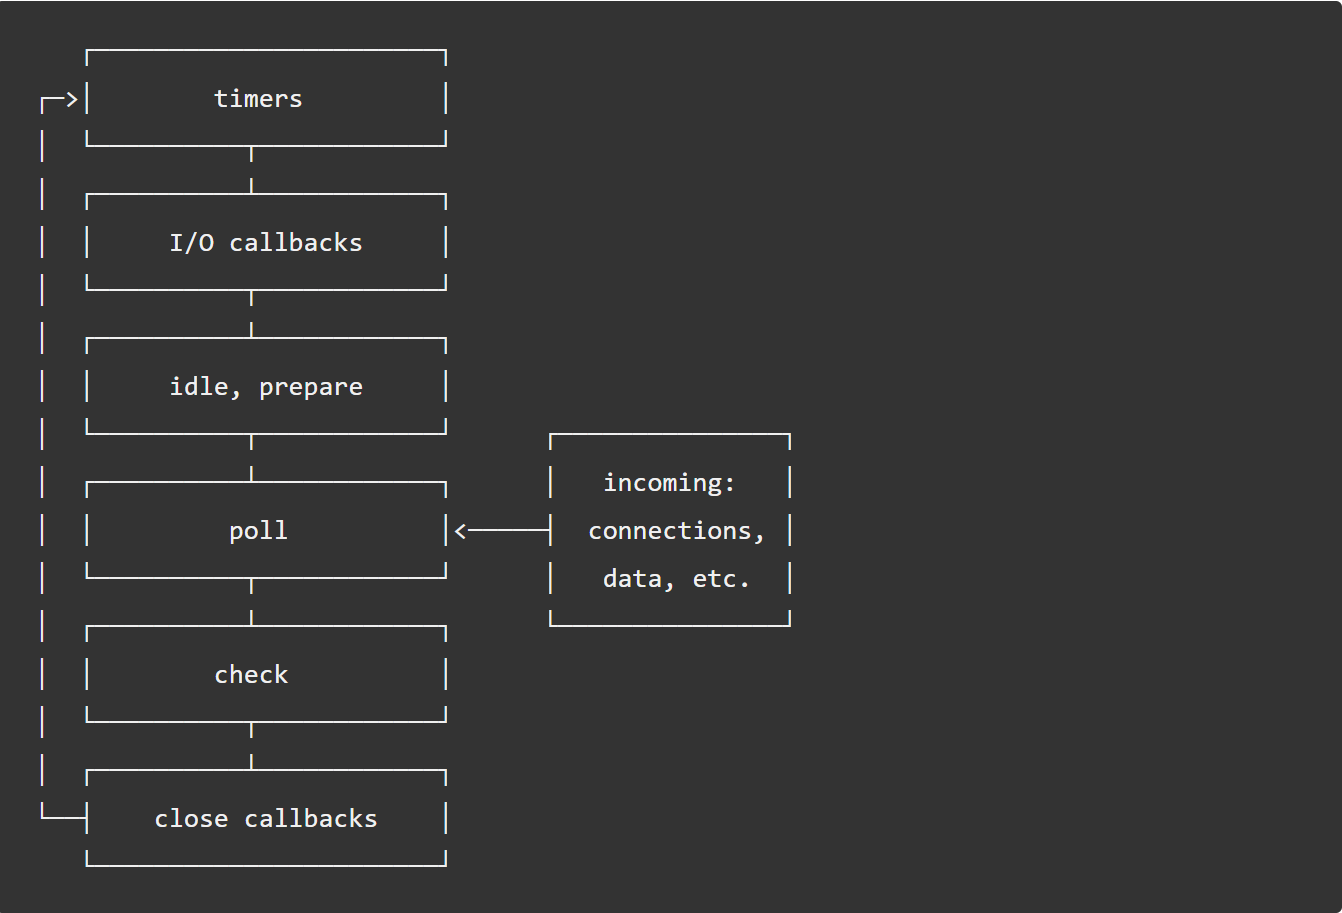
\includegraphics[width=\textwidth]{img/eventLoop.PNG}
\caption{Node Event Loop stages}
\label{fig:eventLoop}
\end{figure}

\noindent For each stage of the event loop there is a first-in-first-out queue of callbacks waiting to be executed. Upon entry of a stage within' the event loop, operations which are specific to that stage are carried out, then callbacks are executed on the stage's queue until either it has been fulfilled entirely, or the callback limit has been reached, once that is done the event loop will proceed to the next stage, et cetera\cite{node}. As these operations can schedule other operations or new events to be processed in the poll stage, which can carry out events as new events are polled. The outcome of this is that the poll phase may go on much longer than a timer's inception. The stages are as follows:
\begin{enumerate}
\item \textbf{Timers:}
	\begin{itemize}
	\item Controlled by the poll stage the timer outlines an opening at which point a provided callback can be executed, as opposed to an exact time someone desires it to be done. Once a certain time frame has gone by, timer callbacks will run. Although they could be delayed by other callbacks or Operating system scheduling. \emph{"Note: To prevent the poll phase from starving the event loop, libuv (the C library that implements the Node.js event loop and all of the asynchronous behaviors of the platform) also has a hard maximum (system dependent) before it stops polling for more events."}\cite{node}
	\end{itemize}
\item \textbf{I/O Callbacks:}
	\begin{itemize}
	\item In the I/O Callbacks stage, system operations callbacks like TCP errors for example, are executed, most callbacks are executed except close callbacks, those scheduled by timers, and set immediate calls .\cite{node}
	\end{itemize}
\item \textbf{Idle, prepare:}
	\begin{itemize}
	\item This is only used internally.\cite{node}
	\end{itemize}
\item \textbf{Poll:}
	\begin{itemize}
	\item The poll stage will execute scripts for timers where their opening has closed, and process events within the poll queue. If there are no timers scheduled upon entry of the poll stage either the event loop will go over its  callbacks queue, executing each one after another in a synchronous manner until all callbacks have been executed, or a limit is reached, if the poll queue is populated. Alternatively if the poll queue is not populated either the poll stage will be ended by the event loop and the check stage begin, or the event loop will wait until callbacks are added to the queue then immediately execute them.\cite{node} When the poll queue has been emptied the event loop will then check for timers whose openings have ended. If this is the case for one or many, the event loop will then return to the timers stage and execute its callbacks.
	\end{itemize}
\item \textbf{Check:}
	\begin{itemize}
	\item In this stage any \verb|setImmediate()| callbacks will be invoked. Also: \emph{"This phase allows a person to execute callbacks immediately after the poll phase has completed."}\cite{node}.
	\end{itemize}
\item \textbf{Close callbacks:}
	\begin{itemize}
	\item Here \verb|process.nextTick()| will be called, but what is that exactly? In Node, each iteration of the event loop is called a "tick". The  \verb|process.nextTick()| function is specific to the Node event loop and when it is used a callback function runs immediately after the events in an event queue have been processed by an iteration of the event loop.  \verb|process.nextTick()| is similar to JavaScript's \verb|setTimeout()| function but operates much faster as it does not have to use JavaScript's runtime to schedule its queue of events.
	\end{itemize}
\end{enumerate}

%%%%%%%%%%%%%%%%%%%%%%%%%%%%%%%%%%%%%%%%%%%%%%%%%%
% Section - TypeScript
%%%%%%%%%%%%%%%%%%%%%%%%%%%%%%%%%%%%%%%%%%%%%%%%%%
\section{TypeScript}
\subsection{What is TypeScript?}
TypeScript\cite{typescript} is a superset of JavaScript which compiles to plain JavaScript. It delivers everything and more that JavaScript has to offer and is a multi-paradigm language that brings flavours of Object-Oritentated Programming and the modern JavaScript Functional Programming techniques together. TypeScript provides a number of benefits when working in a JavaScript environment such as:

\begin{itemize}
\item{Classes:} \\
ECMAScript 6 or ES6 introduced class definitions officially to the JavaScript ecosystem. TypeScript classes are similar however garnished with type checking bring a cleaner, more consistent and robust codebase. 
\item{Interfaces:} \\
The ability to define contracts in one's code and conform to a specified interface provides structure and shape that values adhere to. While a Class may offer a factory or singleton\cite{Gamma:1995:DPE:186897} pattern providing initialisation to values TypeScript interfaces simply define a structural contract that defines what the properties of an object should have as a name and as a type.
\item{Inheritance:} \\
With the use of TypeScript Classes and Interfaces, Inheritance is also provided and gives developers a more comfortable object-orientated approach in designing software and modeling data. Using the extends keyword in object-orientated programming languages such as Java can often be taken for granted and is truly a powerful mechanism in the way in which software is designed.
\item{Static Typing:} \\
The use of Static Typing within TypeScript is a massive bonus for developers both coming from common JavaScript and indeed other statically typed languages such as Java. Static typing or strong typing means that the type of a variable is known at compile time. In contrast, weakly typed or dynamically typed languages associate the type with runtime and as a result types do not need to be specified.
\end{itemize}

And indeed perhaps one of the biggest benefits is enabling IDEs to provide a richer environment for spotting common errors as you write code, which can be one of the most frustrating aspects of writing common JavaScript.

\subsection{Integration with Node.js}

%%%%%%%%%%%%%%%%%%%%%%%%%%%%%%%%%%%%%%%%%%%%%%%%%%
% Section - Databases
%			The Model
%			PostgreSQL & CouchDB 2
%%%%%%%%%%%%%%%%%%%%%%%%%%%%%%%%%%%%%%%%%%%%%%%%%%
\section{Databases}
\subsection{PostgreSQL}
\subsection{CouchDB} %shell scripting
\subsection{Radicale}

%%%%%%%%%%%%%%%%%%%%%%%%%%%%%%%%%%%%%%%%%%%%%%%%%%
% Section - Microsoft Bot Framework
%%%%%%%%%%%%%%%%%%%%%%%%%%%%%%%%%%%%%%%%%%%%%%%%%%
\section{Microsoft Bot Framework}

%Questionable???? Probably should include something for this
%%%%%%%%%%%%%%%%%%%%%%%%%%%%%%%%%%%%%%%%%%%%%%%%%%
% Section - JSON - JSON wrapper for radicale XML
%			JWT?
%%%%%%%%%%%%%%%%%%%%%%%%%%%%%%%%%%%%%%%%%%%%%%%%%%
\section{JSON}
\subsection{Overview}
	The JavaScript Object Notation (JSON) object is a text-based, versatile data interchange format, derived from ECMAScript Programming Language Standard. JSON describes formatting rules for portable representations of data structures\cite{crockford}. It can neither be called nor constructed, and does not contain any major functionality\cite{ecma}. JSON is capable of representing objects, arrays, and other primitive data types such as boolean, numbers, strings, or null\cite{crockford}.  A JSON object would take a form similar to the following example:
\begin{lstlisting}
{
  "student" : {
	"name" : "Jake Johnson",
	"course" : {
		"name" : "Computer Science",
		"year" : 3,
		"modules" : [ "O.O.P.", "O.S.", "Web Apps" ],
		}
  	}
}
\end{lstlisting}
\subsection{Functions}
The JSON object contains functions \emph{parse} and \emph{stringify}, used to parse or construct JSON text. 
\begin{enumerate}
\item \textbf{parse} This function will parse a JSON formatted string and return its ECMAScript value. \emph{"The JSON format is a restricted form of ECMAScript literal. JSON objects are realized as ECMAScript objects. JSON arrays are realized as ECMAScript arrays. JSON strings, numbers, booleans, and null are realized as ECMAScript Strings, Numbers, Booleans, and null."\cite{crockford}}
\item \textbf{stringify} This function will take a ECMAScript value and return a string representation of the object in JSON format. \cite{crockford}
\end{enumerate}
\subsection{Grammer}
JSON and ECMAScript source text are relatively similar. JSON is built up of a series of characters which adhere to the guidelines of SourceCharacter. There are two forms of JSON grammer:
\begin{enumerate}
\item \textbf{Lexical} \emph{"JSON Lexical Grammar defines the tokens that make up a JSON text similar to the manner that the ECMAScript lexical grammar defines the tokens of an ECMAScript source text."\cite{ecma}} 
\item \textbf{Syntactic} \emph{"JSON Syntactic Grammar defines a valid JSON text in terms of tokens defined by the JSON lexical grammar. The goal symbol of the grammar is JSONText."\cite{ecma}}
\end{enumerate}



\section{XML}

%%%%%%%%%%%%%%%%%%%%%%%%%%%%%%%%%%%%%%%%%%%%%%%%%%
% Section - Conclusion
% Maybe leave this conclusion to the very end???
%%%%%%%%%%%%%%%%%%%%%%%%%%%%%%%%%%%%%%%%%%%%%%%%%%
\section{Conclusion}
